% !TeX program = xelatex
% Compile: tectonic --reruns 2 slides/tong_quan_phuong_phap.tex
%
% Overview deck for the project:
%   - dataset, parser, chunking methods, results
%   - deep dive Row-JSON (row_json) and Chipper
%   - how to reproduce the experiments
%
% Data sources:
%   data/eval/three_methods.json
%   data/eval/colpali_results.json
%   data/eval/gold_pages.json
%   data/eval/extraction_gap.json
% Synthesis: docs/Tong_hop_3_phuong_phap_Chunking_va_ColPali.md
\documentclass[aspectratio=169,11pt]{beamer}

% ---- Fonts: prefer Windows fonts, fall back to TeX defaults ----
\usepackage{fontspec}
\IfFontExistsTF{Arial}
  {\setsansfont{Arial}}
  {\IfFontExistsTF{TeX Gyre Heros}
     {\setsansfont{TeX Gyre Heros}}
     {\setsansfont{Latin Modern Sans}}}
\IfFontExistsTF{Times New Roman}
  {\setmainfont{Times New Roman}}
  {\IfFontExistsTF{TeX Gyre Termes}
     {\setmainfont{TeX Gyre Termes}}
     {\setmainfont{Latin Modern Roman}}}
\IfFontExistsTF{Consolas}
  {\setmonofont{Consolas}}
  {\IfFontExistsTF{DejaVu Sans Mono}
     {\setmonofont{DejaVu Sans Mono}}
     {\setmonofont{Latin Modern Mono}}}

\usepackage{amsmath}
\usepackage{booktabs}
\usepackage{array}
\usepackage{tikz}
\usetikzlibrary{arrows.meta,positioning,calc}

\usetheme{Madrid}
\usecolortheme{beaver}
% ``beaver'' is not an xcolor name (Beamer only defines it internally),
% so define it explicitly for TikZ and \color.
\definecolor{brand}{HTML}{7B4B2A}
\setbeamercolor{structure}{fg=brand}
\setbeamertemplate{navigation symbols}{}
\setbeamertemplate{itemize item}{\color{brand!80!black}$\bullet$}
\setbeamertemplate{section in toc}[sections numbered]

\newcommand{\code}[1]{\texttt{\detokenize{#1}}}
\newcommand{\keyidea}[1]{%
  \begin{center}\begin{block}{\small Key takeaway}\centering #1\end{block}\end{center}}
\newcolumntype{L}[1]{>{\raggedright\arraybackslash}p{#1}}

\title[Methods Overview]{Methods Overview: Parsing, Chunking, and Evaluation}
\subtitle[Vietnamese ETF Reports]{Same parser, same gold set --- only the retrieval unit changes}
\author{}
\date{}

\begin{document}

% =============================================================
\begin{frame}
  \titlepage
  \vspace{-1.2em}
  {\footnotesize
  \textbf{Scope:} 7 PDFs / 27 pages / 130 gold questions; parser \code{unstructured}
  \code{hi_res}; CPU, no paid API.\\
  \textbf{Data sources:} \code{data/eval/three_methods.json},
  \code{data/eval/colpali_results.json}, \code{data/eval/gold_pages.json}.}
\end{frame}

% =============================================================
\begin{frame}{Outline}
  \tableofcontents
  \vfill
  {\footnotesize
  Four parts: context and overview $\rightarrow$ deep dive
  \textbf{Row-JSON} $\rightarrow$ deep dive \textbf{Chipper} $\rightarrow$
  how to reproduce the experiments.}
\end{frame}

% =============================================================
\section{Overview}

\begin{frame}{Problem and dataset}
  \begin{columns}[T]
    \begin{column}{0.48\textwidth}
      \begin{block}{Problem}
        \begin{itemize}\footnotesize
          \item Borderless numeric tables in Vietnamese financial/ETF reports.
          \item Gold question: ``what is the value for ticker X?''
          \item Goal: compare retrieval units on one parser; the comparison
            isolates chunking.
        \end{itemize}
      \end{block}
    \end{column}
    \begin{column}{0.48\textwidth}
      \begin{block}{Dataset}
        \begin{itemize}\footnotesize
          \item 7 PDFs: 3 broker forecast reports + 4 SSI bulletins;
            27 pages; 10 gold tables.
          \item 130 questions, 10--40 per file; PDFs have a text layer,
            not scans.
          \item Parser-independent page gold: 111 one-page, 18 two-page,
            1 three-page.
        \end{itemize}
      \end{block}
    \end{column}
  \end{columns}

  \begin{alertblock}{Parser coverage --- read before the results}
    \footnotesize
    \code{unstructured} keeps \textbf{126/130 = 96.9\%} of values at element
    level; \textbf{122/130 = 93.8\%} at chunk level.
    All four misses are missing cell values, not whole rows.
  \end{alertblock}

  {\scriptsize
  \textbf{Evaluation:} chunk-level BM25 (ranking within each file); page-level
  max-pool over 27 pages; Recall@k + MRR; CPU only. Gold QA comes from the
  archived parser's table cells and is kept fixed to measure data lost when
  switching parsers.}
\end{frame}

% =============================================================
\begin{frame}{What parses the PDF: one pipeline}
  \begin{center}
  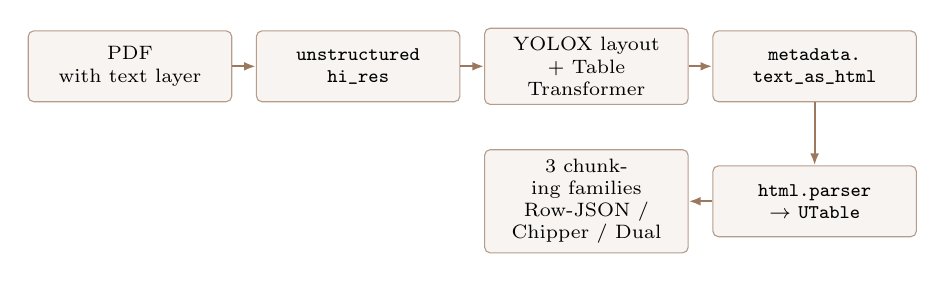
\begin{tikzpicture}[
      node distance=4mm and 3mm,
      box/.style={draw=brand!55, rounded corners=2pt, fill=brand!6,
        align=center, font=\scriptsize, minimum height=9mm,
        text width=2.35cm},
      arrow/.style={-{Latex[length=1.5mm]}, thick, draw=brand!75}]
    \node[box] (pdf) {PDF\\with text layer};
    \node[box, right=of pdf] (unstr) {\code{unstructured}\\ \code{hi_res}};
    \node[box, right=of unstr] (tt) {YOLOX layout\\+ Table Transformer};
    \node[box, right=of tt] (html) {\code{metadata.}\\\code{text_as_html}};
    \node[box, below=8mm of html] (parser) {\code{html.parser}\\$\rightarrow$ \code{UTable}};
    \node[box, left=of parser] (chunkers) {3 chunking families\\Row-JSON / Chipper / Dual};
    \draw[arrow] (pdf) -- (unstr);
    \draw[arrow] (unstr) -- (tt);
    \draw[arrow] (tt) -- (html);
    \draw[arrow] (html) -- (parser);
    \draw[arrow] (parser) -- (chunkers);
  \end{tikzpicture}
  \end{center}

  \begin{columns}[T]
    \begin{column}{0.49\textwidth}
      \begin{block}{Parse call}
        \small
        \code{partition_pdf(strategy="hi_res",}\\
        \code{infer_table_structure=True,}\\
        \code{languages=["vie"])}
      \end{block}
    \end{column}
    \begin{column}{0.49\textwidth}
      \begin{block}{Key points}
        \begin{itemize}\small
          \item Tables come from \code{text_as_html}, not coordinates or
            ruling lines.
          \item \code{PyMuPDF} is used only for page gold and ColPali rendering.
          \item \code{row_json} does not parse PDFs; it only consumes \code{UTable}.
        \end{itemize}
      \end{block}
    \end{column}
  \end{columns}
\end{frame}

% =============================================================
\begin{frame}{From table HTML to \code{UTable}}
  \begin{columns}[T]
    \begin{column}{0.53\textwidth}
      \begin{block}{Four normalization steps}
        \begin{enumerate}\footnotesize
          \item \code{html.parser.HTMLParser} reads \code{<tr>}/\code{<td>}.
          \item Expand \code{colspan}/\code{rowspan} into a rectangular grid.
          \item Header: prefer \code{<thead>}/\code{<th>}; otherwise infer
            from the numeric-cell ratio; join levels with \code{" / "}.
          \item Drop trailing empty columns; attach the nearest preceding
            title/caption.
        \end{enumerate}
      \end{block}
    \end{column}
    \begin{column}{0.43\textwidth}
      \begin{block}{Shared output}
        {\small\ttfamily
        UTable(\\
        \hspace*{1em}columns=["Ticker", "Weight"],\\
        \hspace*{1em}rows=[["MBB", "7.18\%"], ...],\\
        \hspace*{1em}page=2, caption="Table 1: ...")}
      \end{block}
    \end{column}
  \end{columns}

  \vspace{0.2em}
  \begin{block}{Why this step matters}
    \footnotesize
    All three chunking families receive the same \code{UTable}. The only
    difference left is how the table is split, not how the PDF was parsed.
  \end{block}

  {\footnotesize
  \textbf{Warning:} Table Transformer header/merge errors flow straight into
  JSON keys; the 4/130 missing values are a parser limit, not a chunking bug.}
\end{frame}

% =============================================================
\begin{frame}{Methods used}
  \begin{center}
  \scriptsize
  \setlength{\tabcolsep}{4pt}
  \renewcommand{\arraystretch}{1.15}
  \begin{tabular}{@{}L{0.14\textwidth}L{0.28\textwidth}rL{0.17\textwidth}L{0.24\textwidth}@{}}
    \toprule
    \textbf{Family} & \textbf{Splitting rule} & \textbf{\#chunks} &
      \textbf{Returned unit} & \textbf{Best for} \\
    \midrule
    \textbf{Row-JSON} & one table row = one JSON object & 332 &
      one row & cell lookup \\
    \textbf{Chipper} & 4 rules; whole table = 1 chunk & 136 &
      2k chunk / whole table & table context \\
    \textbf{Dual} & small sentences/rows + large passages & 935 &
      large passage or row & small2big \\
    BM25 page & \code{unstructured} text, no chunking & 27 &
      page & baseline \\
    ColPali & page image, zero-shot & 27 &
      page & page triage / scans \\
    \bottomrule
  \end{tabular}
  \end{center}

  \begin{itemize}\footnotesize
    \item All three text methods share \textbf{809 elements and 14 Table
      elements} (10 gold tables); chunk counts differ because the units differ.
    \item \code{chipper_prefix} is a Chipper variant: add the first 2 sentences
      or the caption to the chunk; no LLM.
  \end{itemize}

  \begin{center}\footnotesize
    \textbf{Only the splitting unit changes; parser and retriever stay fixed.}
  \end{center}
\end{frame}

% =============================================================
\begin{frame}{Methods: pros / cons and suitable questions}
  \begin{center}
  \scriptsize
  \setlength{\tabcolsep}{4pt}
  \renewcommand{\arraystretch}{1.18}
  \begin{tabular}{@{}L{0.15\textwidth}L{0.43\textwidth}L{0.38\textwidth}@{}}
    \toprule
    \textbf{Method} & \textbf{Pros / cons} & \textbf{Suitable questions} \\
    \midrule
    \textbf{Row-JSON} &
      \textbf{+} high precision, cheap, self-contained, easy to audit.\newline
      \textbf{$-$} loses whole-table context; cannot aggregate across rows. &
      ``What is MBB's weight?''; compare a few tickers; one-cell lookup. \\
    \textbf{Chipper} &
      \textbf{+} simple, parameter-free, preserves tables, high R@5/R@10.\newline
      \textbf{$-$} whole table becomes one chunk; $\sim$2.3k chars; low R@1. &
      ``What does this table say?''; summarization; LLM context. \\
    \textbf{Dual} &
      \textbf{+} two levels, small2big, reranking.\newline
      \textbf{$-$} many parameters; rerank/dense hurt cell precision. &
      Questions needing passage context; generation; prose. \\
    \textbf{ColPali} &
      \textbf{+} no parser/OCR, sees layout.\newline
      \textbf{$-$} page unit; no cell answer; 256M zero-shot is weak. &
      Scanned PDFs; page selection; fallback when the text layer is lost. \\
    \textbf{BM25 page} &
      \textbf{+} cheap, easy baseline.\newline
      \textbf{$-$} ignores table structure; very weak here. &
      Control baseline. \\
    \bottomrule
  \end{tabular}
  \end{center}

  \begin{center}\footnotesize
    \textbf{No universal best method: the unit must match the question type.}
  \end{center}
\end{frame}

% =============================================================
\begin{frame}{Results}
  \begin{center}
  \scriptsize
  \setlength{\tabcolsep}{3.5pt}
  \renewcommand{\arraystretch}{1.08}
  \begin{tabular}{@{}lrrrrrr@{}}
    \toprule
    \textbf{Method} & \textbf{\#chunks} & \textbf{R@1 chunk} &
      \textbf{R@5 chunk} & \textbf{MRR chunk} & \textbf{R@1 page} &
      \textbf{MRR page} \\
    \midrule
    \textbf{Row-JSON} & 332 & \textbf{81.5\%} & \textbf{90.0\%} &
      \textbf{0.850} & \textbf{90.0\%} & \textbf{0.950} \\
    \code{dual_small} & 935 & 66.1\% & 78.5\% & 0.723 & 73.9\% & 0.844 \\
    \code{dual} & 935 & 50.0\% & 68.5\% & 0.583 & 56.1\% & 0.751 \\
    \code{chipper_prefix} & 136 & 36.9\% & 77.7\% & 0.535 & 45.4\% & 0.665 \\
    \code{dual_dense} & 935 & 31.5\% & 63.8\% & 0.441 & 44.6\% & 0.700 \\
    \code{chipper} & 136 & 27.7\% & 76.9\% & 0.475 & 36.1\% & 0.618 \\
    ColSmol-256M & -- & -- & -- & -- & 13.8\% & 0.288 \\
    BM25 page & -- & -- & -- & -- & 4.6\% & 0.227 \\
    \bottomrule
  \end{tabular}
  \end{center}

  {\scriptsize Sorted by R@1 chunk. \#chunks applies to text methods only;
  page-level max-pool over 27 pages, not 27 chunks.}

  \vspace{0.2em}
  \begin{itemize}\footnotesize
    \item \textbf{Row-JSON} beats \code{dual_small} by 15.4 points R@1 chunk
      and is $\sim$3$\times$ Chipper; page R@1 reaches 90.0\%.
    \item \textbf{Chipper} has R@10 89.2\% but R@1 27.7\%: it
      \emph{contains} the answer but does not rank the cell first.
    \item \textbf{ColPali} 13.8\% page $>$ BM25 4.6\%, but is still
      $\sim$6.5$\times$ below Row-JSON.
  \end{itemize}
\end{frame}

% =============================================================
\begin{frame}{Choose by goal}
  \begin{center}
  \scriptsize
  \setlength{\tabcolsep}{3pt}
  \renewcommand{\arraystretch}{1.10}
  \begin{tabular}{@{}L{0.21\textwidth}L{0.25\textwidth}L{0.46\textwidth}@{}}
    \toprule
    \textbf{Goal} & \textbf{Choose} & \textbf{Why} \\
    \midrule
    Single-cell value / one ticker & \textbf{Row-JSON} + BM25 &
      81.5\% chunk R@1, 90.0\% page R@1; $\sim$491 chars per chunk. \\
    Need whole-table context & Row-JSON + parent table, or Chipper &
      Keep small2big without diluting the cell index. \\
    Qualitative / prose & Dual (large) or a separate prose index &
      Avoid table chunks taking top-1 on numeric questions. \\
    Scanned PDF / no text layer & ColPali after fine-tuning, with GPU &
      256M zero-shot gives only 13.8\% page R@1; not enough to answer. \\
    Academic baseline & Chipper (+ prefix) / BM25 page &
      Parameter-free, reproducible, easy to compare. \\
    \bottomrule
  \end{tabular}
  \end{center}

  \begin{alertblock}{Cross-cutting lesson}
    \footnotesize
    Do not mix all chunk types in one index: BM25 cannot distinguish chunk
    ``contains'' from chunk ``answers''. Adding prose or whole tables to a
    numeric index drops R@1 sharply (\code{dual} 50.0\%, \code{chipper} 27.7\%).
  \end{alertblock}
\end{frame}

% =============================================================
\section{Row-JSON}

\begin{frame}[plain]
  \vfill
  \begin{center}
    {\color{brand}\Large Deep dive 1}\\[0.5em]
    {\Huge\bfseries Row-JSON}\\[0.45em]
    {\large \code{row_json} --- one table row = one JSON object}
  \end{center}
  \vfill
  \begin{block}{Guiding question}
    \centering
    Why does ``one row = one chunk'' win on cell questions?
  \end{block}
\end{frame}

% =============================================================
\begin{frame}{Row-JSON: one table row, one object}
  \begin{columns}[T]
    \begin{column}{0.53\textwidth}
      \begin{block}{One row --- one self-contained object}
        {\scriptsize\ttfamily
        \{"file": "VN30 bulletin Q2/2026",\\
        \hspace*{1em}"page": 2,\\
        \hspace*{1em}"table": "Table 1: ...",\\
        \hspace*{1em}"row": \{"Ticker": "MBB",\\
        \hspace*{4em}"New weight": "7.18\%"\}\}}
      \end{block}
      {\footnotesize Illustrative; real keys come from the table header
      (often Vietnamese in this corpus).}
    \end{column}
    \begin{column}{0.43\textwidth}
      \begin{block}{Why it works}
        \begin{itemize}\small
          \item Entity + value live in \textbf{the same chunk}.
          \item Header is repeated $\rightarrow$ BM25 matches column names.
          \item File/page/caption are self-contained metadata.
          \item Deterministic, no LLM, no GPU; easy to audit.
        \end{itemize}
      \end{block}
    \end{column}
  \end{columns}

  \begin{alertblock}{Naming}
    \small
    Slides call it \textbf{Row-JSON}; code calls it \code{row_json}.
    This is \emph{not} JSONL: one \textbf{table row} is one object, not one
    file line.
  \end{alertblock}

  {\footnotesize
  332 chunks across 7 documents; $\sim$491 chars per chunk. Only rows with
  at least one number become chunks.}
\end{frame}

% =============================================================
\begin{frame}{Path of one row}
  \begin{columns}[T]
    \begin{column}{0.44\textwidth}
      \begin{block}{From PDF to chunk}
        \begin{enumerate}\small
          \item \code{parse_unstructured.py} $\rightarrow$ cache of elements + HTML.
          \item \code{uelements.parse_table_html} $\rightarrow$ \code{UTable}.
          \item \code{row_json_chunks} iterates \code{table.rows}.
          \item \code{table_row_json} $\rightarrow$ JSON for each row.
        \end{enumerate}
      \end{block}
      {\footnotesize
      \code{row_json} does not read PDFs or use coordinates; it only consumes
      the reconstructed table.}
    \end{column}
    \begin{column}{0.52\textwidth}
      \begin{block}{Use as a library}
        {\scriptsize\ttfamily
        from etflab.uelements import load\_unstructured\_doc\\
        from etflab.chunking\_methods import row\_json\_chunks\\[0.35em]
        doc = load\_unstructured\_doc(path)\\
        chunks = row\_json\_chunks(doc, doc["elements"])\\
        print(chunks[0].text)}
      \end{block}
    \end{column}
  \end{columns}

  \vspace*{-0.5em}
  \begin{itemize}\footnotesize
    \setlength{\topsep}{0pt}
    \setlength{\itemsep}{0pt}
    \setlength{\parskip}{0pt}
    \item Rows without numbers are skipped; header/empty rows create no chunk.
    \item No table splitting, no row merging: one row = one event.
    \item If \code{text_as_html} is empty, there is no HTML table
      $\rightarrow$ no chunks.
  \end{itemize}
\end{frame}

% =============================================================
\begin{frame}{Row-JSON: pros / cons}
  \begin{columns}[T]
    \begin{column}{0.48\textwidth}
      \begin{block}{Pros}
        \begin{itemize}\footnotesize
          \item Highest R@1 among text methods: 81.5\% chunk / 90.0\% page.
          \item Small chunks ($\sim$491 chars), focused signal.
          \item Self-contained context: file, page, caption, column names.
          \item No model, no GPU; low ingest cost.
        \end{itemize}
      \end{block}
    \end{column}
    \begin{column}{0.48\textwidth}
      \begin{block}{Cons}
        \begin{itemize}\footnotesize
          \item Loses global table structure: multi-row questions need a
            parent table.
          \item Rows without numbers are dropped; descriptive rows may disappear.
          \item Parser header/cell errors flow straight into JSON keys.
          \item Does not answer qualitative prose questions.
        \end{itemize}
      \end{block}
    \end{column}
  \end{columns}

  \vfill
  {\footnotesize
  \textbf{Strongest point:} a row contains entity, value, and metadata.
  \quad\textbf{Weakest point:} no whole-table context.}
\end{frame}

% =============================================================
\begin{frame}{Row-JSON: suitable questions}
  \begin{columns}[T]
    \begin{column}{0.48\textwidth}
      \begin{exampleblock}{Use when}
        \begin{itemize}\footnotesize
          \item ``What is MBB's weight?''
          \item ``Compare the weights of X and Y'' (top-k rows).
          \item ``Value for Q2.''
          \item ``Is this ticker in the basket?''
        \end{itemize}
      \end{exampleblock}
    \end{column}
    \begin{column}{0.48\textwidth}
      \begin{alertblock}{Do not use alone}
        \begin{itemize}\footnotesize
          \item ``Sum of five tickers.''
          \item ``Trend across the whole table.''
          \item ``Why did the index change?''
        \end{itemize}
      \end{alertblock}
    \end{column}
  \end{columns}

  \vfill
  {\footnotesize
  For multi-row questions: retrieve top-k rows, then expand to the parent table
  or a prose chunk. Do not expect one row to answer an aggregation.}
\end{frame}

% =============================================================
\begin{frame}{Row-JSON: results and limits}
  \begin{columns}[T]
    \begin{column}{0.40\textwidth}
      \begin{block}{Results}
        \centering
        \small
        \begin{tabular}{@{}lrr@{}}
          \toprule
          & \textbf{Chunk} & \textbf{Page} \\
          \midrule
          R@1  & 81.5\% & 90.0\% \\
          R@3  & 90.0\% & 100\% \\
          R@5  & 90.0\% & 100\% \\
          R@10 & 90.0\% & 100\% \\
          MRR  & 0.850 & 0.950 \\
          chars@1 & 494 & -- \\
          \bottomrule
        \end{tabular}
      \end{block}
    \end{column}
    \begin{column}{0.56\textwidth}
      \begin{block}{Why does it stop at 90\%?}
        \begin{itemize}\small
          \item Coverage 93.8\% (122/130): 4 values missing in parser output,
            4 entity/value pairs split across chunks.
          \item R@3 = R@10 = 90.0\%: 8 questions outside coverage, 5 have an
            answer but are outside top-3.
          \item 4 misses: TCB 8.75\%, TPB 3,729, MBB 65,517, MBB 24.4.
        \end{itemize}
      \end{block}
    \end{column}
  \end{columns}

  \vspace{0.2em}
  \begin{alertblock}{To go beyond 90\%}
    \small
    Fix the parser (header/merge) or add parent-table expansion. Tuning BM25
    cannot recover the 4 values absent from parser output.
  \end{alertblock}
\end{frame}

% =============================================================
\section{Chipper}

\begin{frame}[plain]
  \vfill
  \begin{center}
    {\color{brand}\Large Deep dive 2}\\[0.5em]
    {\Huge\bfseries Chipper}\\[0.45em]
    {\large element-based chunking, arXiv:2402.05131}
  \end{center}
  \vfill
  \begin{block}{Guiding question}
    \centering
    Why does a method that follows the paper still underperform on numeric tables?
  \end{block}
\end{frame}

% =============================================================
\begin{frame}{Chipper: model or method?}
  \begin{alertblock}{Two things often confused}
    \small
    \textbf{Chipper} is the name of a \emph{layout model} (Unstructured's
    vision encoder-decoder).\quad
    The \textbf{method} in the paper is \textbf{element-based chunking}.
    This project uses the \emph{method}, not the Chipper model.
  \end{alertblock}

  \begin{columns}[T]
    \begin{column}{0.48\textwidth}
      \begin{block}{Paper}
        \begin{itemize}\small
          \item Four rules, no parameters; 2,048-char threshold.
          \item FinanceBench (10-K/10-Q), English.
          \item Goal: ``best chunk size without tuning''.
        \end{itemize}
      \end{block}
    \end{column}
    \begin{column}{0.48\textwidth}
      \begin{block}{Project}
        \begin{itemize}\small
          \item Same \code{unstructured} element stream.
          \item 136 chunks; tables kept whole.
          \item \code{chipper_prefix}: add first 2 sentences / caption.
          \item No GPT-4, no API.
        \end{itemize}
      \end{block}
    \end{column}
  \end{columns}

  \begin{center}\footnotesize
    \textbf{This is a reproducible baseline, not a comparison of the Chipper model.}
  \end{center}
\end{frame}

% =============================================================
\begin{frame}{Chipper's four rules}
  \begin{enumerate}\small
    \item \textbf{Follow the reading order} of elements.
    \item \textbf{Pack up to 2,048 chars}; never split an element.
    \item \textbf{Title} $\rightarrow$ start a new chunk (title stays in the new chunk).
    \item \textbf{Table} $\rightarrow$ start a new chunk and \textbf{keep the whole table}.
  \end{enumerate}

  \begin{center}
  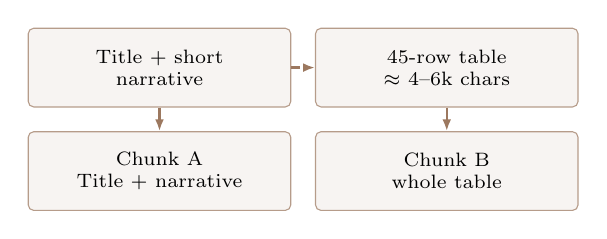
\begin{tikzpicture}[
      node distance=3mm,
      box/.style={draw=brand!55, rounded corners=2pt, fill=brand!6,
        align=center, font=\scriptsize, minimum height=10mm,
        text width=3.1cm},
      arrow/.style={-{Latex[length=1.5mm]}, thick, draw=brand!75}]
    \node[box] (a) {Title + short\\narrative};
    \node[box, right=of a] (b) {45-row table\\$\approx$ 4--6k chars};
    \node[box, below=of a] (c) {Chunk A\\Title + narrative};
    \node[box, below=of b] (d) {Chunk B\\whole table};
    \draw[arrow] (a) -- (c);
    \draw[arrow] (b) -- (d);
    \draw[arrow, dashed] (a) -- (b);
  \end{tikzpicture}
  \end{center}

  \begin{alertblock}{Consequence}
    \footnotesize
    A 45-row table remains \textbf{one chunk}, even far above 2,048 chars.
    That is rule 4, not an implementation bug. Chipper chunks are often
    ``the whole table'', so BM25 has one coarse signal.
  \end{alertblock}
\end{frame}

% =============================================================
\begin{frame}{Application and pros / cons}
  \begin{columns}[T]
    \begin{column}{0.50\textwidth}
      \begin{block}{Application on \code{unstructured}}
        \begin{itemize}\footnotesize
          \item Elements: title, narrative, list, table, caption.
          \item Skip header/footer/pagebreak/image/formula.
          \item \code{chipper_prefix}: first 2 sentences (prose) or caption (table).
          \item 136 chunks; average 557 chars (prefix: 662).
        \end{itemize}
      \end{block}
    \end{column}
    \begin{column}{0.46\textwidth}
      \begin{block}{Pros}
        \begin{itemize}\footnotesize
          \item Simple, parameter-free, reproducible.
          \item Keeps tables intact; high R@5/R@10.
          \item Broad context, good for generation.
        \end{itemize}
      \end{block}
      \begin{block}{Cons}
        \begin{itemize}\footnotesize
          \item Whole-table chunk $\sim$2.3k chars, low R@1.
          \item Large tables far exceed 2,048.
          \item Caption/header are not enough to locate a cell.
        \end{itemize}
      \end{block}
    \end{column}
  \end{columns}

  \begin{exampleblock}{Suitable questions}
    \scriptsize
    ``What does this table say?'' $\cdot$ summarization $\cdot$ LLM context.
    \quad\textbf{Not:} ``What is MBB's weight?''.
  \end{exampleblock}
\end{frame}

% =============================================================
\begin{frame}{Chipper: results}
  \begin{center}
  \footnotesize
  \setlength{\tabcolsep}{4pt}
  \renewcommand{\arraystretch}{1.15}
  \begin{tabular}{@{}lrrrrrrr@{}}
    \toprule
    \textbf{Variant} & \textbf{\#chunks} & \textbf{avg chars} &
      \textbf{R@1} & \textbf{R@5} & \textbf{R@10} & \textbf{MRR} &
      \textbf{R@1 page} \\
    \midrule
    \code{chipper} & 136 & 557 & 27.7\% & 76.9\% & 89.2\% & 0.475 & 36.1\% \\
    \code{chipper_prefix} & 136 & 662 & 36.9\% & 77.7\% & 89.2\% & 0.535 & 45.4\% \\
    \bottomrule
  \end{tabular}
  \end{center}

  {\footnotesize
  \code{chars@1}: 2,299 (chipper) and 2,430 (prefix) --- $\sim$4.7--4.9$\times$
  Row-JSON. R@10 nearly matches Row-JSON, but R@1 is only $\sim$1/3.}

  \begin{itemize}\footnotesize
    \item Prefix improves \textbf{+9.2 points R@1 chunk} and
      \textbf{+9.3 points R@1 page}; it is still 44.6 points behind Row-JSON.
    \item R@10 89.2\% is evidence of ``contains'' but not ``answers'':
      the table is in top-10, rarely first.
    \item Typical failures: 45-row tables; lost captions; adjacent tables
      merged; numbers in headers confuse BM25.
  \end{itemize}

  \keyidea{Chipper is a context builder, not a cell locator.}
\end{frame}

% =============================================================

% =============================================================
\section{Dual-granularity}

\begin{frame}[plain]
  \vfill
  \begin{center}
    {\color{brand}\Large Deep dive 3}\\[0.6em]
    {\huge\bfseries Dual-granularity}\\[0.4em]
    {\large \texttt{dual\_small}, \texttt{dual}, \texttt{dual\_dense} --- small-to-big}
  \end{center}
  \vfill
  \begin{block}{Guiding question}
    \centering
    Why does returning the \textbf{whole table} hurt cell lookup?
  \end{block}
\end{frame}

% =============================================================
\begin{frame}{Dual-granularity: small-to-big idea}
  \begin{columns}[T]
    \begin{column}{0.48\textwidth}
      \begin{block}{Two levels from same elements}
        \begin{itemize}\footnotesize
          \item \textbf{Large} (\code{dual\_large}): prose grouped by \code{title} up to
            \code{large\_target}; \textbf{each table becomes a single large chunk}.
          \item \textbf{Small}: derived from large. For numeric table rows ->
            \code{dual\_row} (with \code{parent\_id}); for prose ->
            sentences/groups.
          \item Linked by \code{parent\_id}.
        \end{itemize}
      \end{block}
    \end{column}
    \begin{column}{0.48\textwidth}
      \begin{block}{Small-to-big retrieval}
        \begin{itemize}\footnotesize
          \item \textbf{Search on small}: find precise location.
          \item \textbf{Expand to parent}: return large chunk for context.
          \item Balance \textbf{precision} (small) + \textbf{context} (large).
        \end{itemize}
      \end{block}
    \end{column}
  \end{columns}

  \vspace{0.3em}
  \begin{alertblock}{Same retriever}
    \footnotesize
    Only \textbf{indexed set} and \textbf{returned chunk} differ. BM25 + doc-filter unchanged.
  \end{alertblock}
\end{frame}

% =============================================================
\begin{frame}{\code{dual\_small} vs \code{dual} vs \code{dual\_dense}}
  \begin{center}
  \footnotesize
  \setlength{\tabcolsep}{4pt}
  \renewcommand{\arraystretch}{1.15}
  \begin{tabular}{@{}p{0.16\textwidth}p{0.24\textwidth}p{0.52\textwidth}@{}}
    \toprule
    \textbf{Variant} & \textbf{Index / Return} & \textbf{Description} \\
    \midrule
    \code{dual\_small} & small only / small &
      Search \code{dual\_row} + \code{dual\_small}. Return small chunk. Best for
      ``value of ticker X''. \\
    \midrule
    \code{dual} & small / large (parent) &
      Find on small, expand to \code{dual\_large}. For tables this is
      \textbf{the whole table}. \\
    \midrule
    \code{dual\_dense} & small / large + \code{e5-small} &
      Same as \code{dual}, with sentence merging + dense rerank. Helps prose,
      hurts rigid numeric tables. \\
    \bottomrule
  \end{tabular}
  \end{center}
\end{frame}

% =============================================================
\begin{frame}{Why returning the whole table hurts}
  \begin{columns}[T]
    \begin{column}{0.48\textwidth}
      \begin{block}{Cell queries}
        \begin{itemize}\footnotesize
          \item \code{dual\_small}: hits exact \code{dual\_row} with ticker+value.
          \item \code{dual}: must rank inside a 45-row table -> diluted.
          \item \code{dual\_dense}: reranking favors broader semantic matches.
        \end{itemize}
      \end{block}
    \end{column}
    \begin{column}{0.48\textwidth}
      \begin{block}{Chunk-level (130 questions)}
        \footnotesize
        \setlength{\tabcolsep}{4pt}
        \renewcommand{\arraystretch}{1.15}
        \begin{tabular}{@{}lrrrrr@{}}
          \toprule
          \textbf{Variant} & \textbf{\#chunks} & \textbf{R@1} & \textbf{R@5} & \textbf{R@10} & \textbf{MRR} \\
          \midrule
          \code{dual\_small} & 935 & 66.1\% & 78.5\% & 86.2\% & 0.723 \\
          \code{dual} & 935 & 50.0\% & 68.5\% & 68.5\% & 0.583 \\
          \code{dual\_dense} & 935 & 31.5\% & 63.8\% & 63.8\% & 0.441 \\
          \bottomrule
        \end{tabular}
      \end{block}
      \begin{block}{Takeaway}
        \footnotesize
        Small-to-big is good when parent adds context. Bad when parent = entire table.
      \end{block}
    \end{column}
  \end{columns}
\end{frame}

% =============================================================
\begin{frame}{Dual vs Row-JSON vs Chipper}
  \begin{columns}[T]
    \begin{column}{0.48\textwidth}
      \begin{block}{When to use}
        \begin{itemize}\footnotesize
          \item \textbf{Prose/narrative}: explanations benefit from context.
          \item \textbf{Mixed docs}: need both small precision and big context.
          \item \textbf{Hybrid strategy}: put table cells in tight units; keep prose in Dual if needed.
        \end{itemize}
      \end{block}
    \end{column}
    \begin{column}{0.48\textwidth}
      \begin{block}{Chunk-level R@1}
        \footnotesize
        \setlength{\tabcolsep}{4pt}
        \renewcommand{\arraystretch}{1.15}
        \begin{tabular}{@{}lr@{}}
          \toprule
          \textbf{Method} & \textbf{R@1} \\
          \midrule
          \code{row\_json} & \textbf{81.5\%} \\
          \code{dual\_small} & 66.1\% \\
          \code{dual} & 50.0\% \\
          \code{chipper\_prefix} & 36.9\% \\
          \code{dual\_dense} & 31.5\% \\
          \code{chipper} & 27.7\% \\
          \bottomrule
        \end{tabular}
      \end{block}
      \begin{alertblock}{Bottom line}
        \footnotesize
        For ``value of ticker X'', \textbf{keep unit small}. \code{row\_json} best overall;
        \code{dual\_small} second among dual; returning whole table hurts badly.
      \end{alertblock}
    \end{column}
  \end{columns}
\end{frame}

\end{document}
